% !TEX root = thesis.tex
\chapter{Design Methodology}
\label{sec:design_methodology}

This chapter presents the design methodology used to extend the Spiker+ framework with hardware support for \gls{sdsp}-based online learning. The original Spiker+ architecture provides a configurable hardware generation flow for \gls{fpga}-based \gls{snn}s, but the synaptic weights used by the generated accelerator are primarily prepared through offline training and remain unchanged during network operation \cite{Carpegna2025}.

To enable online learning, the existing inference architecture must be extended so that synaptic weights can be modified according to the activity of the network. This requires more than the addition of an isolated learning circuit. The neuron states required by the \gls{sdsp} rule must be made available to the learning logic, the synaptic weight storage must support runtime write operations, and the inference and learning processes must be coordinated to avoid inconsistent memory accesses.

The proposed methodology therefore begins with an analysis of the original Spiker+ data and control flow. Based on this analysis, a hardware-oriented \gls{sdsp} module is designed and connected to the neuron and synapse-processing path. The overall design aims to preserve the modular structure of Spiker+ while introducing the additional state variables, interfaces, and control operations required for online weight adaptation. The following sections describe the design requirements, the proposed system architecture, the digital implementation of the learning rule, and the integration of the learning functionality into the existing \gls{snn} accelerator.

\section{Design Objectives and Requirements}
\label{subsec: design objectives and requirements}

The central objective of this work is to extend an \gls{snn} accelerator generated by Spiker+ so that its synaptic weights can be updated during network operation. The learning mechanism is based on \gls{sdsp}, for which a presynaptic event triggers a local decision using the current synaptic weight and the state of the corresponding postsynaptic neuron \cite{Brader2007}. The resulting weight change must be retained by the hardware and used when the same synapse is accessed again. Consequently, online learning must become part of the normal data and control flow of the accelerator rather than an independent post-processing step.

The first functional requirement is to preserve the original inference behaviour. Adding the learning path must not change the interpretation of input spikes, the update of the neuron state, or the generation of output spikes. Learning must therefore be controllable independently of inference. When learning is inactive, the accelerator must leave the stored weights unchanged and behave as an inference-only Spiker+ design. When learning is active, the modified weight must influence subsequent synaptic operations without requiring the network to be regenerated or restarted.

The second requirement is architectural compatibility with Spiker+. The existing hierarchy of network, layer, and neuron components should be retained as far as possible so that the learning extension does not remove the configurability of the framework. Instead of replacing the original neuron datapath, the proposed design adds clearly defined interfaces through which the learning logic obtains the required neuron and synapse information. This modular organization also separates the learning decision from the remaining neuron operations and allows both parts to be verified independently.

Correct \gls{sdsp} operation requires the relevant state values to be available at the same time as the synapse being processed. These values include the current synaptic weight, the postsynaptic membrane potential, and an activity-related state representing recent postsynaptic firing. The design must also maintain the association between these values and the addresses of the active pre- and postsynaptic neurons. A weight update applied to an incorrect address would change the behaviour of a different connection and therefore invalidate the learning process.

Online learning also changes the requirements of the synaptic weight storage. Whereas an inference-oriented accelerator can use weights that remain constant after initialization, the proposed system requires a writable storage structure and a controlled write-back path. Weight reads used for synaptic processing and weight writes produced by the learning unit must be performed in a deterministic order. The controller must prevent a new transaction from overwriting or bypassing an unfinished update and must guarantee that later accesses observe the most recently stored weight.

All learning-related quantities must be represented using finite-width digital values. The weight, membrane potential, activity state, and learning thresholds must therefore be mapped to suitable integer or fixed-point representations. The selected width must provide sufficient resolution for the required behaviour while avoiding unnecessary logic and memory consumption. Because the synaptic weight has a finite numerical range, the update must be bounded. Potentiation at the maximum value must not cause overflow, and depression at the minimum value must not cause underflow.

Finally, the learning extension should introduce limited computational overhead and remain suitable for synthesis on the target \gls{fpga}. The hardware-oriented formulation of \gls{sdsp} is advantageous in this respect because its update decision can be implemented mainly with comparisons, additions, subtractions, and control logic rather than multipliers or global gradient calculations \cite{Frenkel2019ODIN}. The added modules and interfaces should remain parameterizable where practical and should expose observable control and state signals for module-level and system-level verification.

Together, these requirements define the design space of the proposed system. The architecture must combine correct local learning, writable and bounded synaptic state, deterministic coordination with inference, and compatibility with the modular Spiker+ structure. The following section uses these requirements to derive the overall architecture of the online-learning accelerator.

\section{Baseline Spiker+ Architecture}
\label{subsec: baseline spikerplus architecture}

Spiker+ generates synthesizable VHDL descriptions from a high-level \gls{snn} configuration. Its hardware architecture is organized hierarchically: a network-level control unit coordinates the complete inference process, each layer has a dedicated controller and synaptic-weight storage, and every neuron is divided into a control unit and a datapath \cite{Carpegna2022,Carpegna2025}. Understanding this hierarchy is necessary before introducing online learning because the required neuron states, weight values, addresses, and synchronization signals are distributed across several modules.

Figure \ref{fig:spikerplus-generated-architecture} reproduces the high-level architecture presented in the Spiker+ paper. The illustrated three-layer feed-forward network is a generic example rather than the exact network instance used in this thesis, but it shows the same structural principles. Red paths carry spike data, green paths provide synaptic weights, and blue paths represent control and synchronization. A Network Control Unit (Network CU) coordinates the layers, each Layer Control Unit (Layer CU) distributes input events, and every neuron contains a Neuron Control Unit (Neuron CU) connected to a Neuron Datapath (Neuron DP).

\begin{figure}[t]
	\centering
	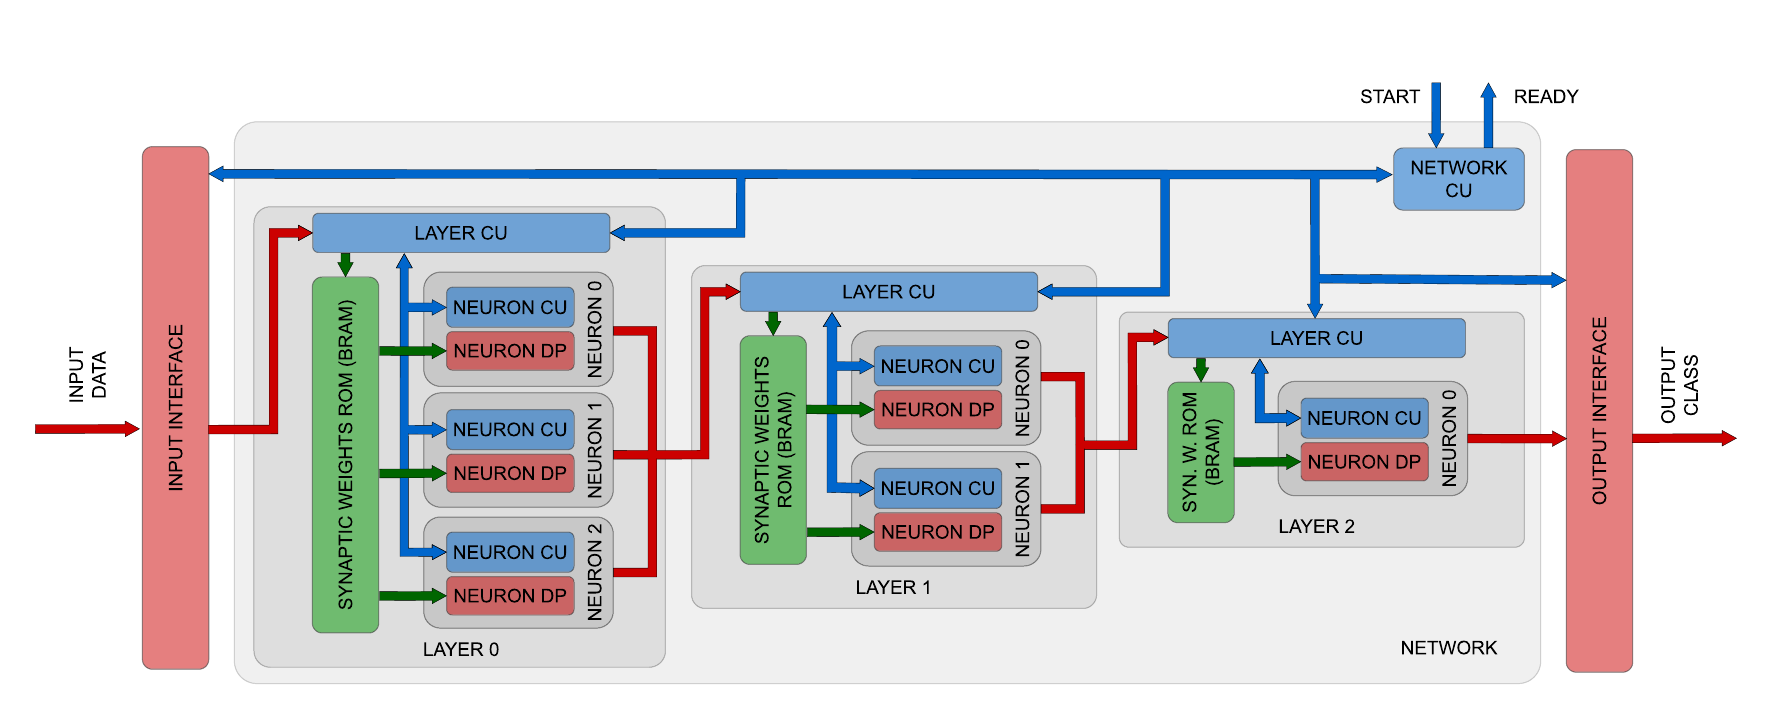
\includegraphics[width=\linewidth]{figures/spikerplus_generated_architecture_original.png}
	\caption{High-level Spiker+ Architecture for a Feed-Forward Fully Connected \gls{snn} \cite{Carpegna2025}}
	\label{fig:spikerplus-generated-architecture}
\end{figure}

\subsection{Architecture Hierarchy and Baseline Instance}

At the accelerator boundary, an input interface converts encoded spike addresses into the internal spike-vector representation expected by the network. In the generated baseline, the \texttt{full\_accelerator} module performs this conversion using a decoder and a bank of input registers. The network output is represented internally as a vector of neuron spikes, while an output multiplexer allows an individual output spike to be selected through the external interface.

The \texttt{network} module instantiates the network controller and the generated layer modules. The Network CU governs the temporal evolution of the \gls{snn} over a configurable number of processing cycles. It distributes a start condition to the layers, waits for their completion signals, and generates a restart signal when the state of the network must be initialized for a new sample.

The baseline instance examined in this work contains 784 external excitatory inputs and a layer of ten output neurons. The output spikes are returned to the same layer as inhibitory inputs, creating recurrent competition between the output neurons. The layer therefore contains separate excitatory and inhibitory input paths, their corresponding weight memories, ten neuron instances, and a barrier that collects the neuron outputs. Although these dimensions are specific to the generated baseline, the same hierarchy is used by Spiker+ for other supported network configurations.

\subsection{Processing and Synchronization}

Spiker+ combines sequential synapse processing with parallel neuron processing. Within a layer, the input controller iterates over the excitatory input addresses and then over the inhibitory inputs. For each address, the corresponding input spike and one weight for every postsynaptic neuron are selected. The ten neurons can consequently process the same presynaptic event in parallel, while the individual presynaptic connections are supplied sequentially. This organization avoids implementing a separate processing datapath for every synapse while retaining parallelism across the neurons of a layer.

Communication between the control levels follows a start/ready handshake. The Network CU starts a network cycle only when the participating layers are ready. At the layer level, the Layer CU initiates the next input operation and waits until the neurons report completion. Their \texttt{neuron\_ready} signals are combined with the barrier status to form the layer-level completion condition. The barrier stores the produced output spikes and prevents the controller from advancing while one or more neuron operations are unfinished.

This synchronization mechanism is directly relevant to online learning. A weight update must remain associated with the input address and postsynaptic neuron that produced the learning decision. The layer must therefore retain the relevant address and state information until the update is complete, and its ready condition must account for any additional learning and write-back latency.

\subsection{Neuron Datapath and Weight Storage}

Each baseline neuron is separated into a finite-state control unit and an arithmetic datapath, as indicated in Figure \ref{fig:spikerplus-generated-architecture}. The controller selects operations for initialization, excitatory integration, inhibitory integration, leakage, firing, and idle behaviour. The datapath stores the membrane potential in a signed register, selects the appropriate update value, performs addition or subtraction, and compares the result with the firing threshold. Leakage is implemented through a shift operation, and firing uses a subtractive reset so that the residual membrane potential is preserved.

In the original neuron interface, the membrane potential remains internal to the datapath. The surrounding layer receives only the output spike and the completion status. This interface is sufficient for inference, but it does not expose the postsynaptic state required by \gls{sdsp}. Integrating the learning rule therefore requires an additional connection between the neuron state and the learning logic without changing the existing inference operations.

The baseline layer stores excitatory and inhibitory weights in separate generated memories. The current input index is used as the read address, and one access returns the weights connected to all ten postsynaptic neurons. This memory organization matches the processing schedule because all neurons operate on the selected presynaptic input in parallel. In the examined design, the membrane potential uses a 16-bit representation and both excitatory and inhibitory weights use three-bit values.

The weight memories are initialized from the parameters produced during offline training. Their generated interfaces contain a clock, a read address, and weight outputs, but no write-enable signal, write data, or runtime update path. The stored values therefore remain constant during inference. This is the principal storage limitation that prevents the baseline accelerator from supporting online learning.

\subsection{Implications for the Learning Extension}

The architecture shown in Figure \ref{fig:spikerplus-generated-architecture} already provides a modular separation between network control, layer control, neuron computation, and synaptic storage. This structure makes it possible to introduce learning without replacing the complete accelerator. Nevertheless, the baseline analysis identifies three required modifications.

First, the postsynaptic membrane potential and the additional activity state required by \gls{sdsp} must be made available outside the original neuron datapath. Second, the static excitatory-weight memory must be replaced or extended with writable storage and a correctly addressed write-back interface. Third, the layer-level control and ready logic must coordinate inference, the learning decision, and completion of the weight update. These requirements guide the architecture developed in the following sections.

\section{Proposed Online-Learning Architecture}
\label{subsec: proposed online learning architecture}

The proposed architecture extends the generated Spiker+ accelerator with a local online-learning path while retaining the original network, layer, and neuron hierarchy. The existing datapath continues to process spikes and update the neuron states, whereas the added path observes the current synaptic and postsynaptic states, evaluates the learning conditions, and writes an updated excitatory weight back to memory. Figure \ref{fig:proposed-online-learning-architecture} presents this relationship at the system level. Blue connections indicate the original inference path, while orange connections show the learning and write-back path introduced in this work.

\begin{figure}[t]
	\centering
	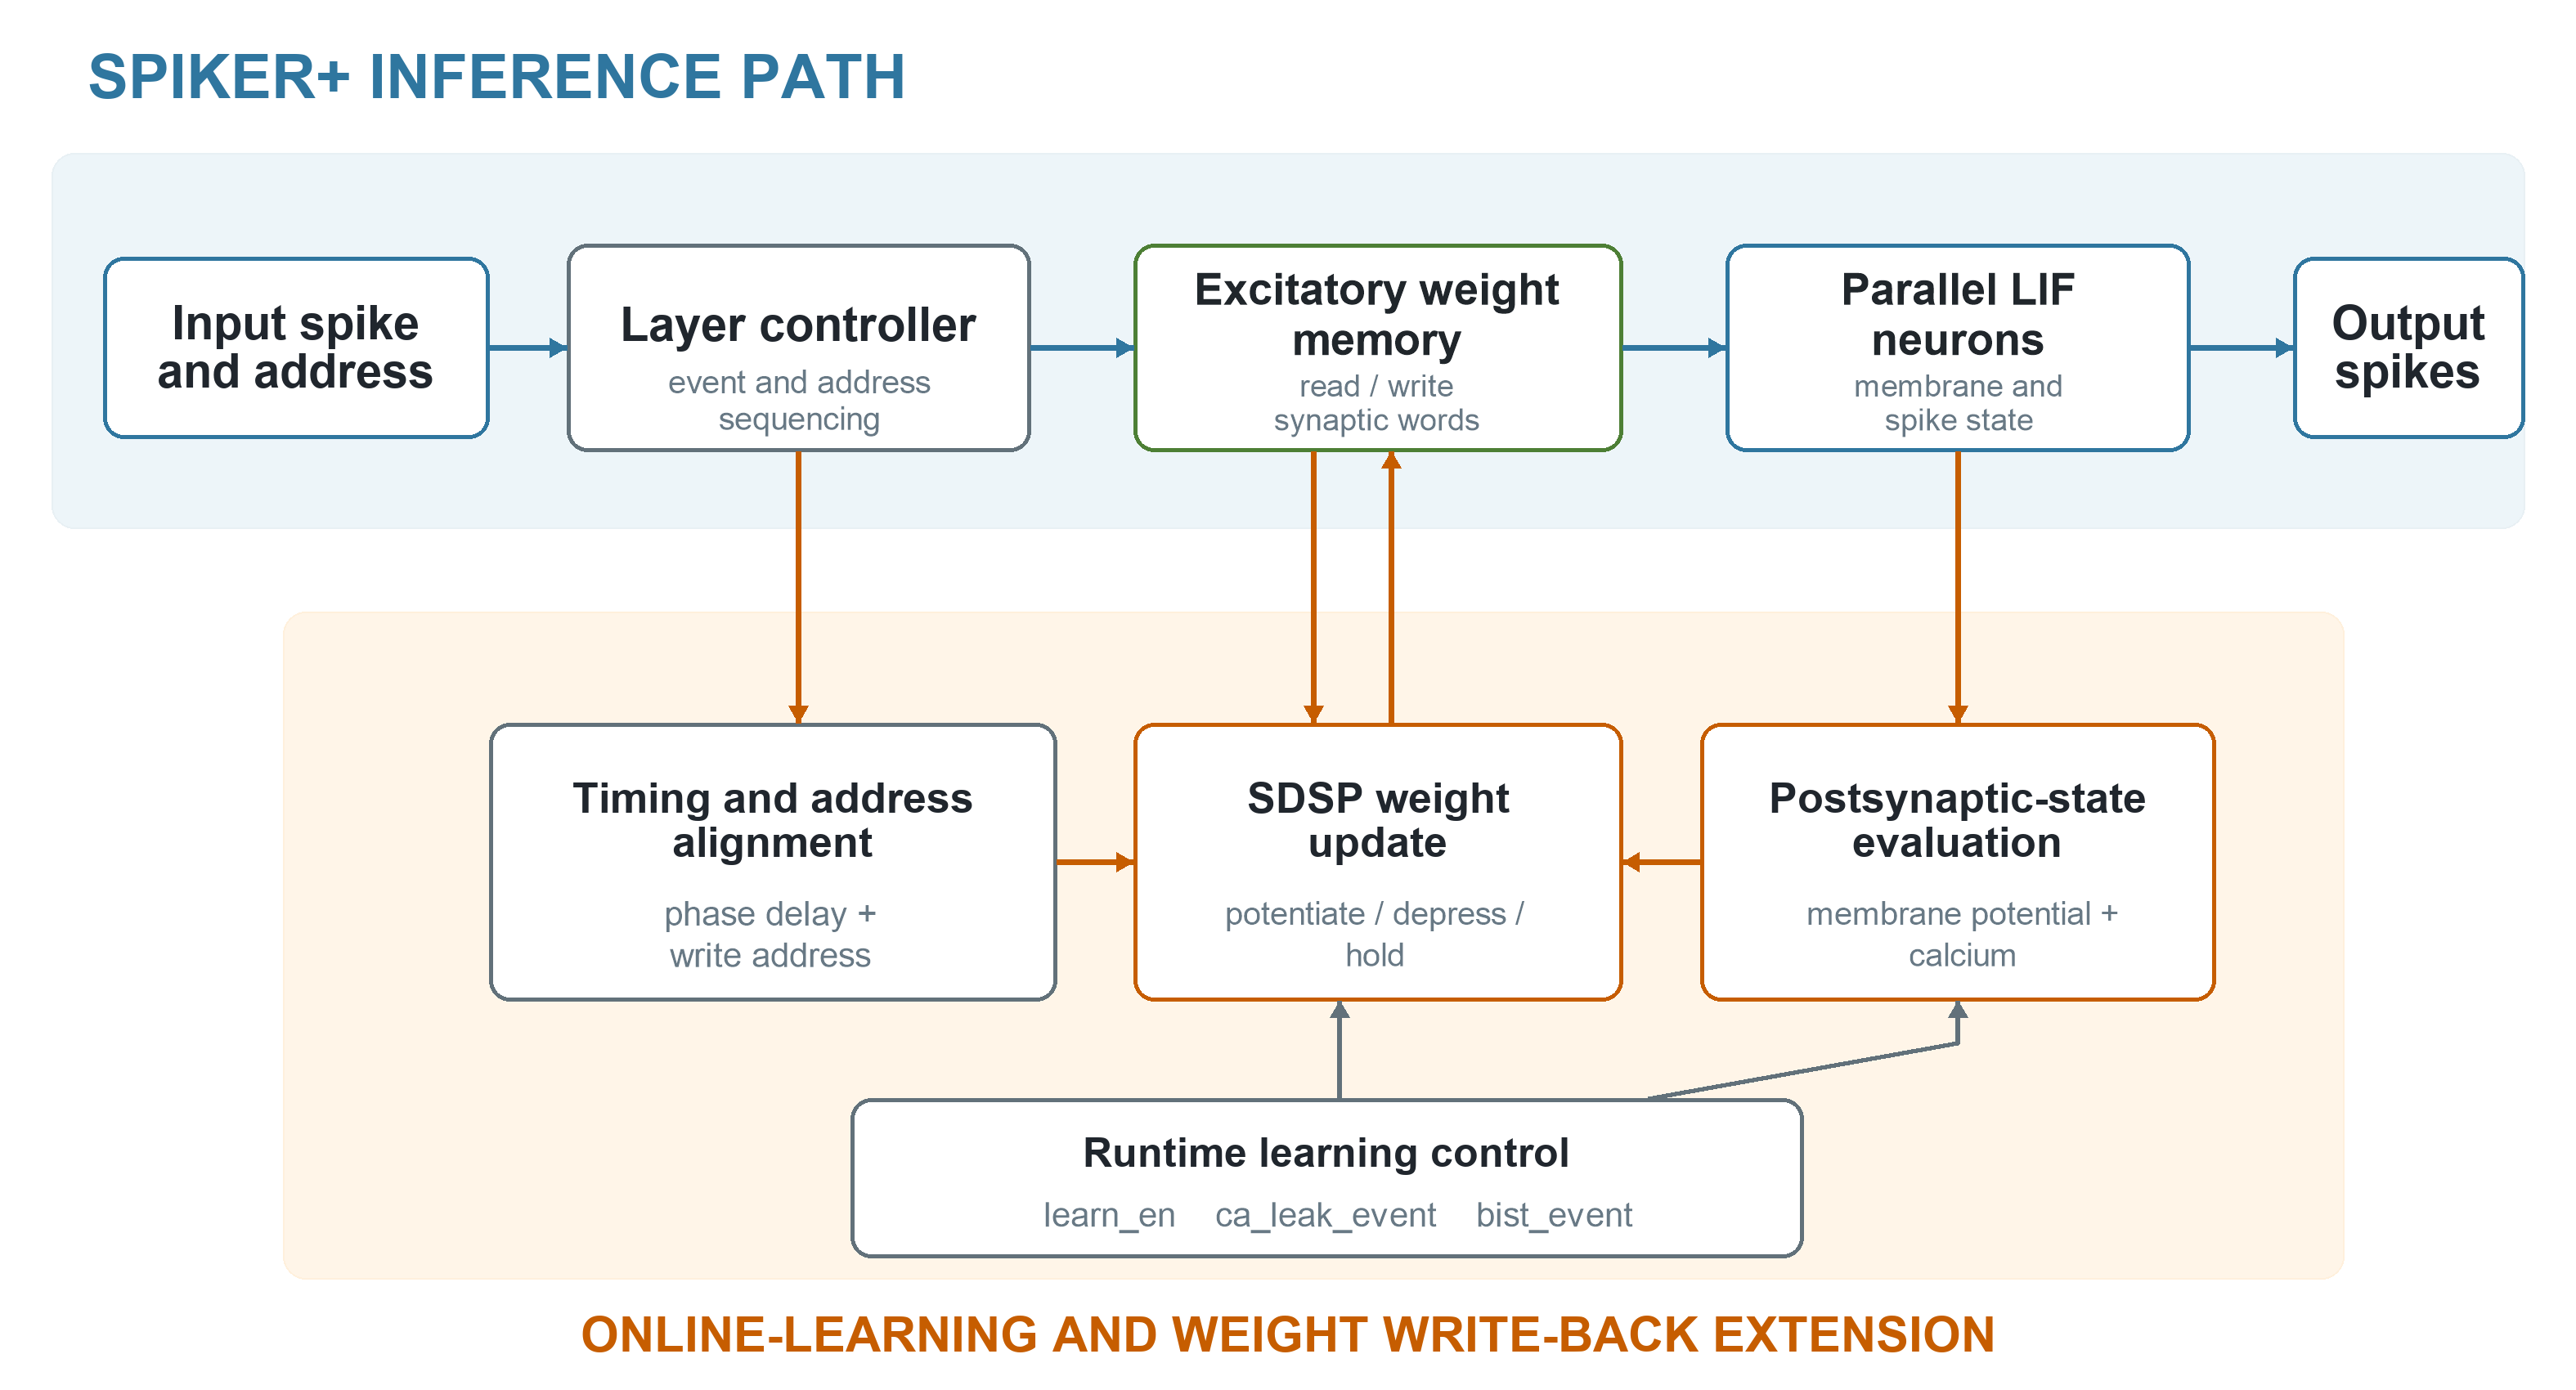
\includegraphics[width=\linewidth]{figures/proposed_online_learning_architecture.png}
	\caption{Integration of the \gls{sdsp} Learning and Weight Write-Back Path into the Spiker+ Architecture}
	\label{fig:proposed-online-learning-architecture}
\end{figure}

\subsection{Overall Organization}

As shown in Figure \ref{fig:proposed-online-learning-architecture}, the network-level controller and the original start/ready coordination remain responsible for executing the generated \gls{snn}. At the layer level, the controller selects a presynaptic address and reads the corresponding synaptic weights. The excitatory weight word is then distributed to the parallel \gls{lif} neuron datapaths, while the fixed inhibitory memory continues to support the recurrent competition between the output neurons. The inference path therefore preserves the processing model of the baseline Spiker+ accelerator \cite{Carpegna2025}.

The principal architectural change is the feedback path from the postsynaptic neurons to the excitatory-weight memory. The modified neuron datapath exposes its membrane potential without changing the existing integration, leakage, firing, or subtractive-reset operations. Each postsynaptic neuron is additionally associated with a calcium counter that represents its recent firing activity. The membrane potential and calcium state are evaluated together to generate the potentiation and depression conditions required by the \gls{sdsp} rule \cite{Brader2007}.

One \gls{sdsp} update unit is instantiated for each postsynaptic neuron. Consequently, all weights contained in the currently read word can be evaluated in parallel, matching the parallel organization of the neuron datapaths. The resulting weight fields are reassembled into an updated word and returned to the excitatory memory. The learning extension is restricted to the feed-forward excitatory synapses; the inhibitory memory and its inference path remain unchanged.

\subsection{Learning and Weight Write-Back Flow}

For every excitatory input transaction, the layer controller supplies a presynaptic event and selects the associated weight word. The same weights are used by the neuron datapaths for synaptic integration and by the learning units as the current synaptic state. In parallel, the learning path receives the postsynaptic membrane potentials, calcium states, and the externally supplied learning-control events. These local quantities determine whether each weight is potentiated, depressed, or retained.

Online learning requires the update to remain associated with the address from which the original weight was read. This is non-trivial because the generated Spiker+ layer prefetches the next weight word while advancing through the presynaptic addresses. The proposed architecture therefore delays the indication of the excitatory processing phase and retains the valid write address. A pending-write signal transfers the update request across the clock boundary so that the completed weight word is written to the correct memory entry. The same mechanism also retains the update belonging to the final excitatory input when the layer controller changes to the next processing phase.

The original read-only excitatory storage is replaced by a writable memory with separate read and write addresses. A read supplies the weights required for the current synaptic operation, while a subsequent write commits the learning result. This organization permits a completed update to be stored while the controller prepares the next input access. Because the entire word is written together, the parallel results produced for all postsynaptic neurons remain synchronized.

During the inhibitory phase, the layer follows the original inference path. Inhibitory weights are read from the unchanged memory and supplied only to the neuron datapaths; no learning request or write-back operation is generated. This separation confines the additional memory and control logic to the synapses that are adapted by the implemented learning rule.

\subsection{Operating Modes and Synchronization}

Three control inputs are added at the accelerator boundary and propagated through the network to the modified layer. The \texttt{learn\_en} signal enables weight updates. When it is disabled, the excitatory-memory write interface remains inactive, the initialized weights are retained, and the accelerator operates in its original inference-only mode. Training and evaluation can therefore be selected at runtime without regenerating the hardware.

The \texttt{ca\_leak\_event} signal controls the decay of the calcium counters independently of the synapse-processing rate. The \texttt{bist\_event} signal activates the bistability mechanism that drives intermediate weights toward stable states. These two events are distributed globally, whereas the membrane potential, calcium state, learning decision, and synaptic weight remain local to the relevant postsynaptic neuron and connection.

The original start/ready synchronization between the network, layer, neurons, and output barrier is retained. The learning request and write-back are aligned with the existing layer schedule by the phase-delay, registered-address, and pending-write logic shown in Figure \ref{fig:proposed-online-learning-architecture}. Therefore, no independent training controller or global learning handshake is required. The modified layer additionally reports when an input event has been accepted and when the corresponding output step is valid, providing precise transaction boundaries for system-level integration and verification.

In summary, the proposed architecture preserves the original event-processing datapath and introduces a local feedback loop for online adaptation. The postsynaptic state determines the learning condition, the presynaptic event identifies the active synaptic word, and the aligned write-back path stores the updated result at the correct address. The next section describes the digital realization of the \gls{sdsp} update function used inside this architecture.

\section{Digital Realization of the SDSP Learning Rule}
\label{subsec: digital sdsp realization}

The digital learning path follows the hardware-oriented organization used in ODIN: the postsynaptic state is evaluated separately from the synaptic weight update, and the resulting direction information is supplied to a compact arithmetic datapath \cite{Frenkel2019ODIN}. The proposed design applies this separation to every postsynaptic neuron while retaining the parallel weight organization of the generated Spiker+ layer.

\subsection{Learning Conditions and Compact Update Flow}

Each postsynaptic neuron is associated with a calcium counter that represents its recent firing activity. A postsynaptic spike increments the counter, whereas \texttt{ca\_leak\_event} decrements it. The counter saturates at its upper and lower limits, holds its value when neither operation is requested, and is cleared at the beginning of a new sample. This follows the interpretation of the calcium state used in the digital \gls{sdsp} implementation of ODIN \cite{Frenkel2019ODIN}.

At the arrival time \(t_{\mathrm{pre}}\) of a presynaptic spike, the current calcium state and membrane potential determine the direction of the possible weight change. The two update cases are expressed as

\begin{equation}
\begin{cases}
w \rightarrow w+1, &
V_{\mathrm{mem}}(t_{\mathrm{pre}}) \geq V_{\mathrm{th}},
\quad \theta_1 \leq C(t_{\mathrm{pre}}) < \theta_3\\
w \rightarrow w-1, &
V_{\mathrm{mem}}(t_{\mathrm{pre}}) < V_{\mathrm{th}},
\quad \theta_1 \leq C(t_{\mathrm{pre}}) < \theta_2
\end{cases}
\label{eq:sdsp-weight-update-conditions}
\end{equation}

Figure \ref{fig:sdsp-weight-update-overview} shows the inputs and outputs of the \gls{sdsp} online-learning module. The comparator evaluates the conditions in Equation \ref{eq:sdsp-weight-update-conditions} and exposes them through the Boolean signals \texttt{up} and \texttt{down}. When \texttt{spk\_pre} is asserted, the update datapath samples these conditions and either increments, decrements, or retains the current weight. If no presynaptic spike is active, the separate \texttt{bistability} input can request an update based on the most significant bit of the current weight. Separating the condition state from the update trigger allows the arithmetic datapath to read only the decision required at the event time. The detailed arithmetic implementation is described in the next subsection.

\begin{figure}[t]
	\centering
	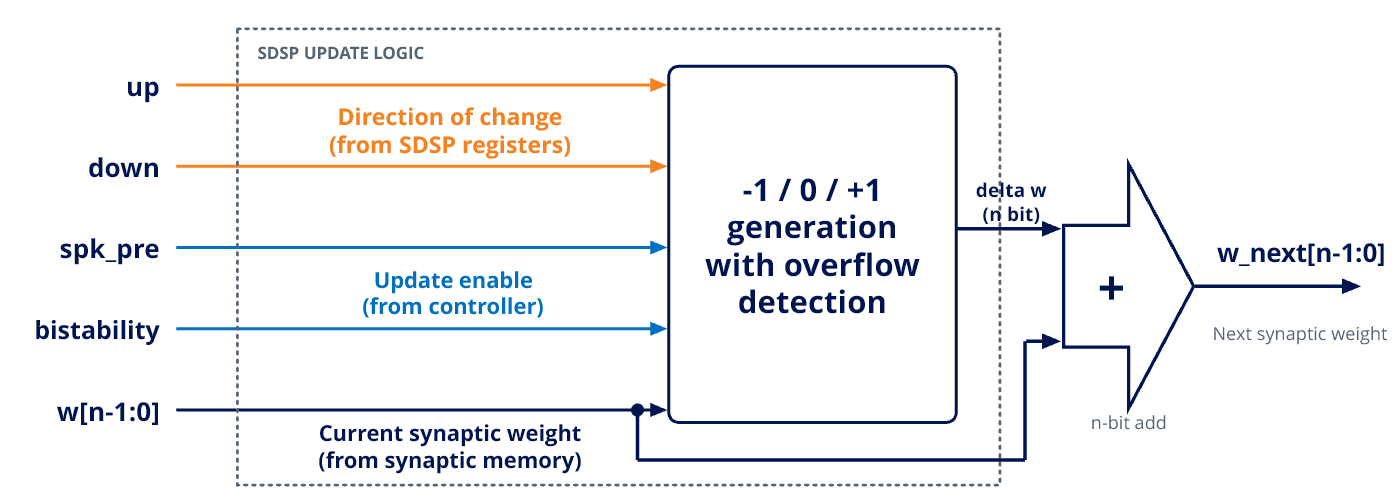
\includegraphics[width=\linewidth]{figures/sdsp_weight_update_overview.png}
	\caption{Control and Arithmetic Organization of the \gls{sdsp} Weight-Update Datapath}
	\label{fig:sdsp-weight-update-overview}
\end{figure}

This organization keeps the learning decision simple. The neuron-side state determines only the direction of change, while the synaptic datapath performs the bounded arithmetic update. It also matches the memory organization of the modified Spiker+ layer: all weights belonging to the selected presynaptic address are read together, and one update datapath evaluates each postsynaptic weight in parallel.

\subsection{Detailed Weight-Update Datapath}

Figure \ref{fig:sdsp-weight-update-datapath} shows the detailed structure of \texttt{sdsp\_top}. The \texttt{delta\_w\_generator} receives \texttt{up}, \texttt{down}, \texttt{spk\_pre}, \texttt{bist}, and the most significant bit of the current weight. It converts the requested operation into the \texttt{delta\_w} word and the carry input \texttt{cin} used by the \(N\)-bit adder.

The generator does not produce a signed arithmetic value such as \(-1\) directly. Instead, addition and subtraction are represented through an \(N\)-bit two's-complement encoding and the carry input of the adder. For an increment, \texttt{delta\_w} is set to all zeros and \texttt{cin} is asserted, so that the adder evaluates \(w_{\mathrm{current}}+0+1\). For a decrement, \texttt{delta\_w} is set to all ones and \texttt{cin} is cleared. The all-one word represents \(2^N-1\), which is equivalent to \(-1\) modulo \(2^N\), and the same unsigned adder therefore evaluates \(w_{\mathrm{current}}-1\). When no update is requested, both outputs are zero and the current weight is passed through unchanged. This encoding explains why both \texttt{delta\_w} and \texttt{cin} are supplied by the generator to the adder: together they express the complete update operation without requiring a separate subtractor or a signed datapath.

\begin{figure}[t]
	\centering
	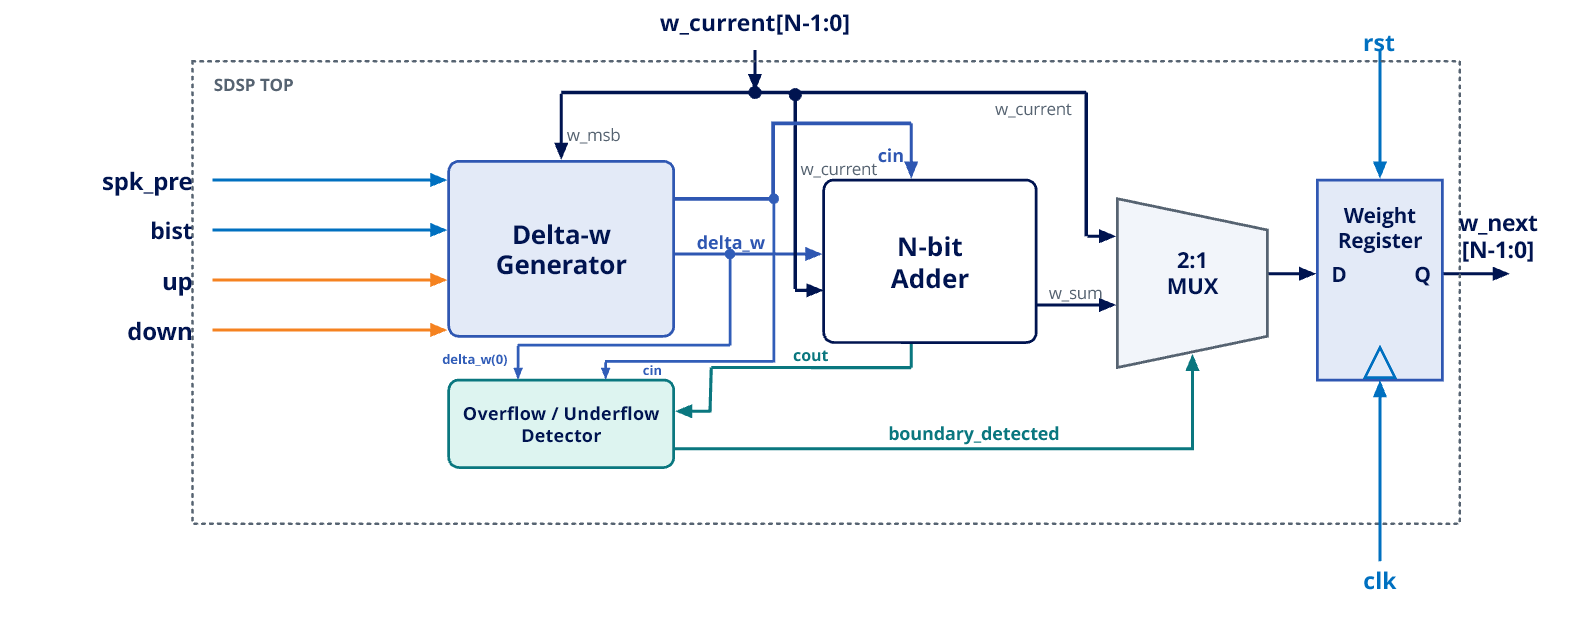
\includegraphics[width=\linewidth]{figures/sdsp_digital_datapath.png}
	\caption{\gls{rtl} Datapath for Bounded \gls{sdsp} Weight Increment and Decrement}
	\label{fig:sdsp-weight-update-datapath}
\end{figure}

For spike-driven learning, \texttt{spk\_pre} has priority and the generator uses the current \texttt{up}/\texttt{down} state. When no presynaptic spike is active, \texttt{bist} can apply the bistability mechanism described for ODIN \cite{Frenkel2019ODIN}. The most significant weight bit identifies the lower or upper half of the numerical range. A bistability event then moves an intermediate weight toward the corresponding low or high stable region.

The adder combines the encoded change with \texttt{w\_current} and produces \texttt{w\_sum} together with the carry output \texttt{cout}. The overflow/underflow detector evaluates \texttt{delta\_w(0)}, \texttt{cin}, and \texttt{cout}. The solid junctions in Figure \ref{fig:sdsp-weight-update-datapath} indicate that the detector inputs branch from the same \texttt{delta\_w} and \texttt{cin} signals used by the adder. If an increment at the maximum value or a decrement at zero would wrap the unsigned weight, \texttt{boundary\_detected} makes the multiplexer retain \texttt{w\_current}. Otherwise, the multiplexer forwards \texttt{w\_sum}. The weight register captures the selected value on the active clock edge and is reset through \texttt{rst}.

One \gls{sdsp} datapath is instantiated for each postsynaptic neuron, and the resulting fields are combined into the complete word written back to the excitatory memory. The arithmetic update therefore remains local, while the address-alignment logic described in Section \ref{subsec: proposed online learning architecture} preserves the association between the updated word and the correct presynaptic input.

\section{Integration into the Spiker+ Accelerator}
\label{subsec:integration-into-spikerplus}

The learning extension is integrated at the layer level because this is the lowest level of the Spiker+ hierarchy at which the presynaptic address, the synaptic weight word, and all postsynaptic neuron states are available together. The network-level scheduler and the original neuron-control sequence are retained \cite{Carpegna2025}. The modified layer adds only the state-observation, update, and memory-write functions required for online learning.

\begin{figure}[t]
	\centering
	\makebox[\linewidth][c]{%
		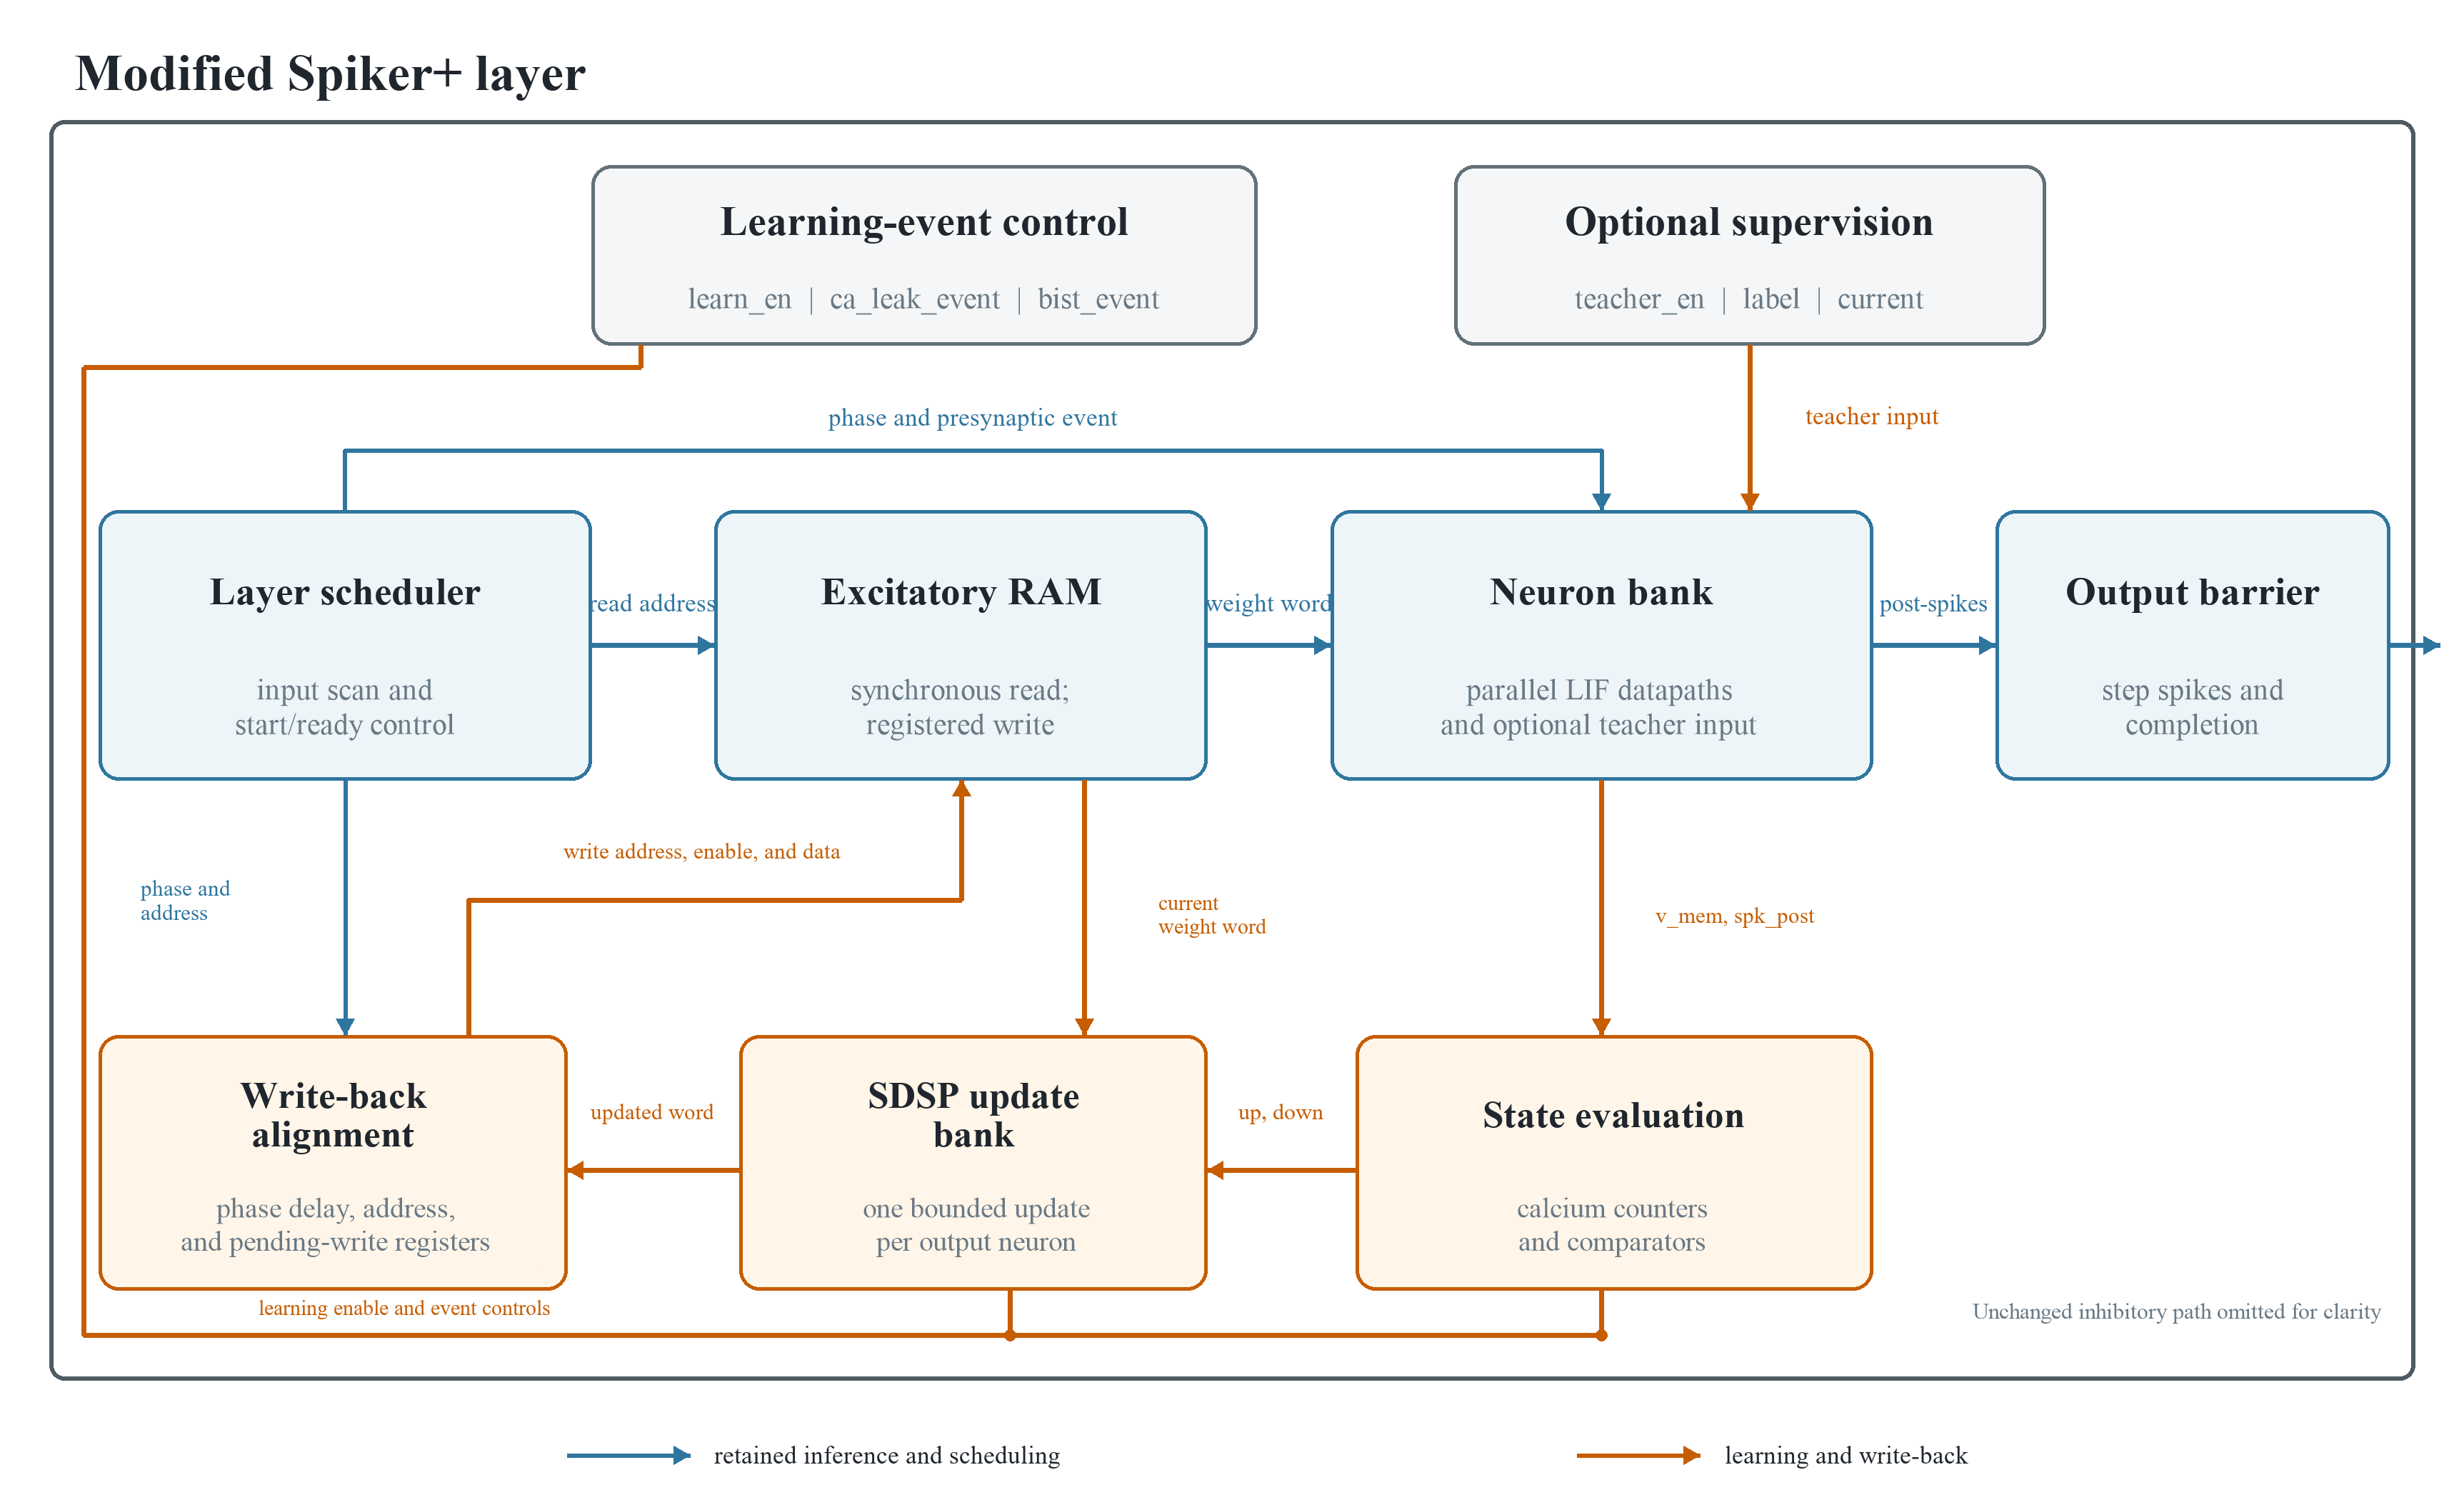
\includegraphics[width=1.06\linewidth]{figures/spiker_sdsp_layer_integration.png}%
	}
	\caption{Layer-Level Integration of the \gls{sdsp} State-Evaluation and Weight Write-Back Paths into Spiker+}
	\label{fig:spiker-sdsp-layer-integration}
\end{figure}

\subsection{Layer-Level Integration and State Formation}

Figure \ref{fig:spiker-sdsp-layer-integration} separates the retained inference path from the added learning feedback path. The layer scheduler continues to scan the excitatory inputs sequentially and supplies the active phase, presynaptic event, and read address. One word from the excitatory memory contains the weights from the selected input to all output neurons. The complete word is therefore delivered to the parallel neuron bank in one access, preserving the processing organization of the generated accelerator. The output barrier and the recurrent inhibitory path are unchanged; the latter is omitted from the figure because it is not modified by the learning extension.

For each output neuron, the current weight is used simultaneously by the neuron datapath and by one \gls{sdsp} update unit. The modified neuron interface exposes the membrane potential and postsynaptic spike. A local calcium counter and comparator convert these quantities into the two update conditions described in Section \ref{subsec: digital sdsp realization}. The same structure is replicated for every output neuron, so all fields in the selected weight word are evaluated in parallel and reassembled into one updated word.

The learning-event interface supplies the global enable, calcium-decay event, and bistability event shown at the top of Figure \ref{fig:spiker-sdsp-layer-integration}. These controls determine when local state is updated and when a weight modification may be committed; they do not replace the normal layer schedule. The final implementation also includes an optional supervision path. At the beginning of each network time step, the configured teacher current is applied only to the output neuron selected by the class label, and only when both supervision and learning are enabled. This current changes the target neuron's membrane state and therefore influences the subsequent local \gls{sdsp} decision. It does not write a weight directly, so weight modification remains governed by the same presynaptic event and postsynaptic-state conditions as the unsupervised path.

\subsection{Address-Aligned Read--Modify--Write Sequence}

Replacing the excitatory read-only storage with writable memory creates a timing problem: the Spiker+ input scanner advances while the synchronous memory prefetches the next weight word. The learning result must nevertheless be written to the address from which its original weight was obtained. Figure \ref{fig:spiker-sdsp-writeback-sequence} summarizes the resulting sequence for an arbitrary excitatory address \(k\).

\begin{figure}[t]
	\centering
	\makebox[\linewidth][c]{%
		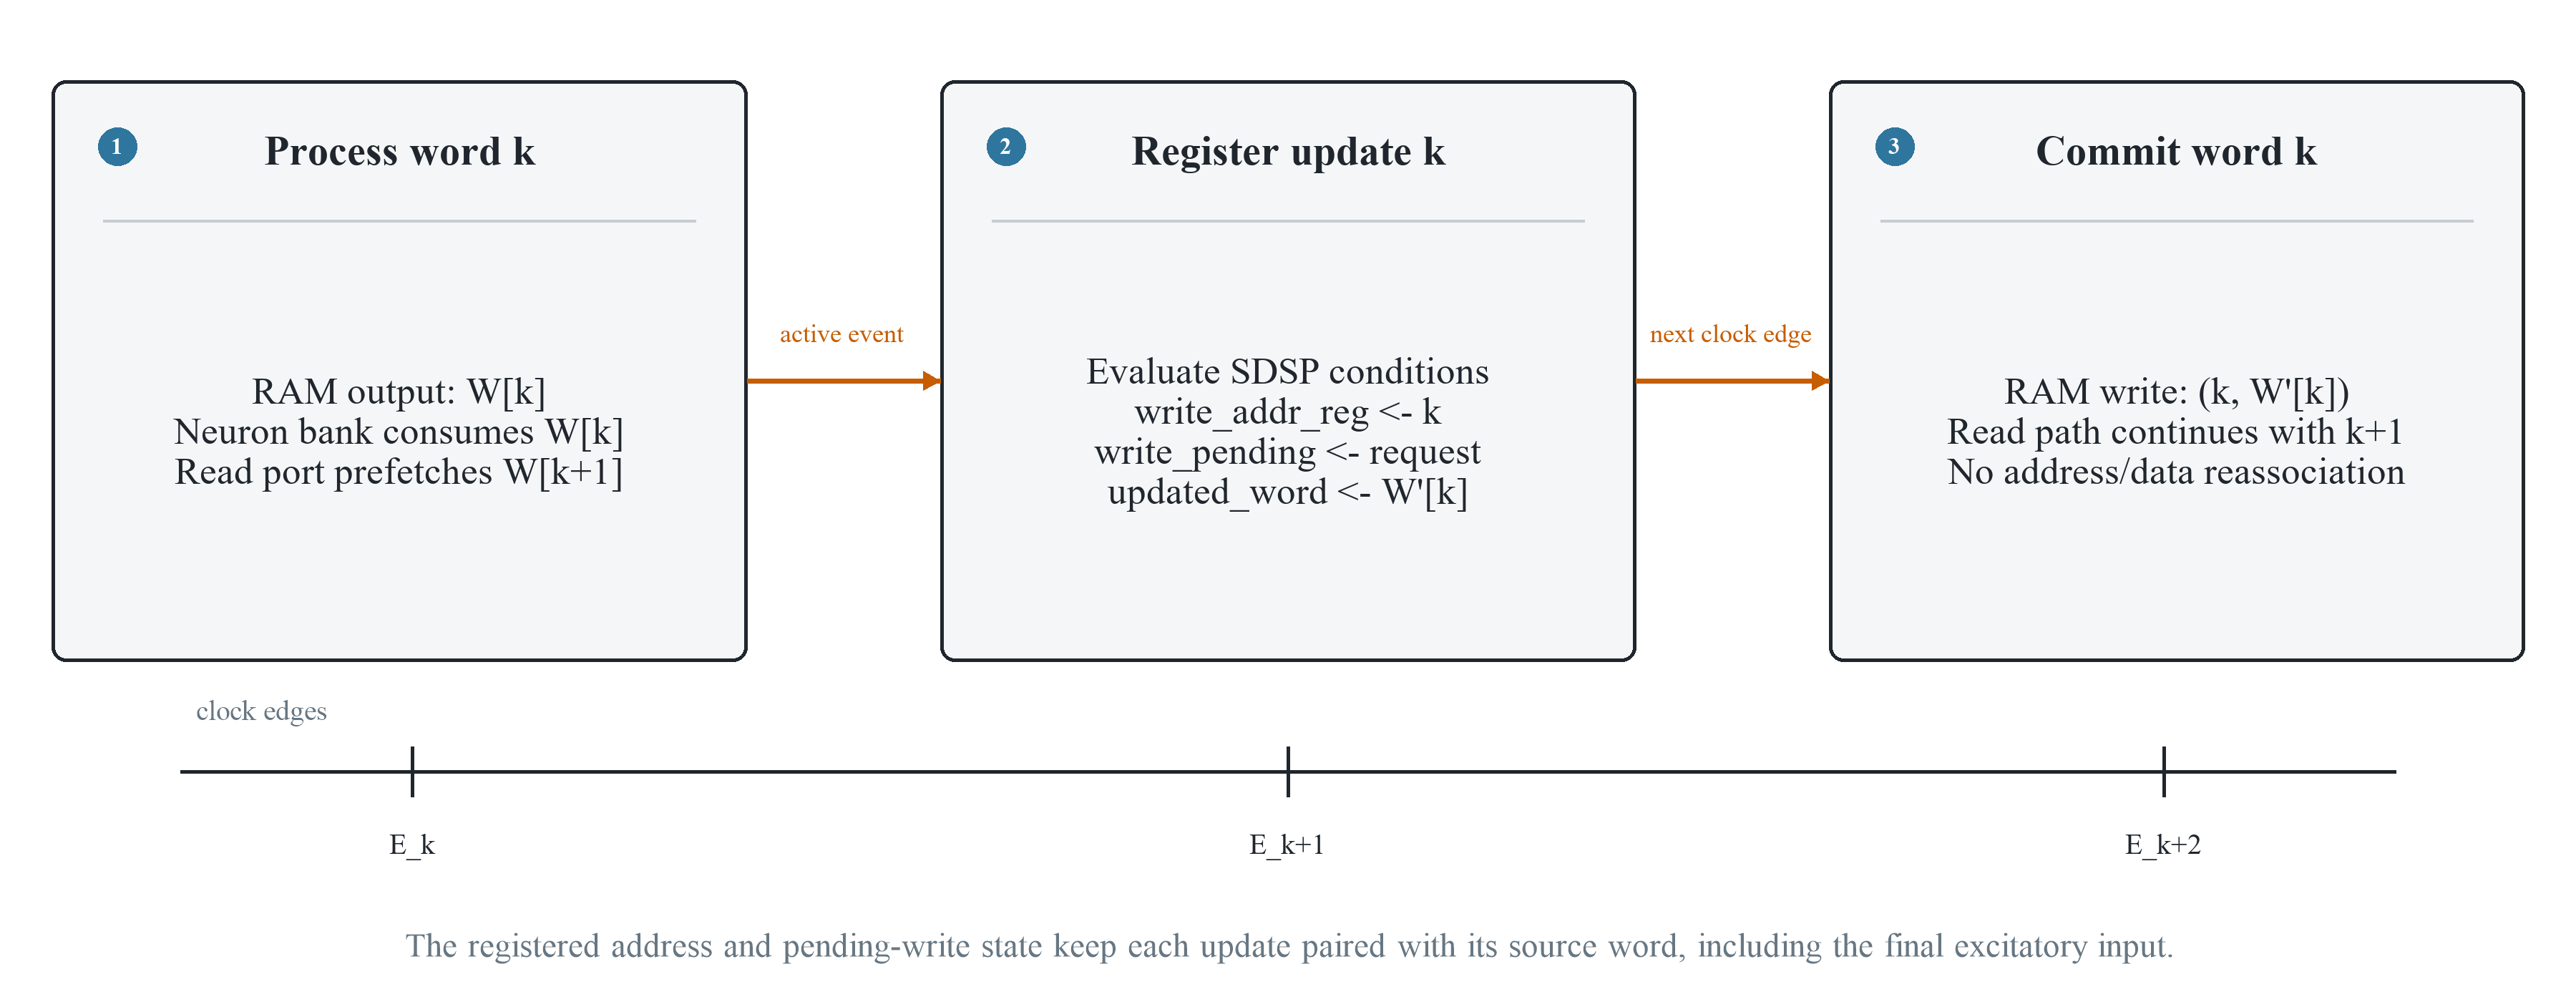
\includegraphics[width=1.05\linewidth]{figures/spiker_sdsp_writeback_sequence.png}%
	}
	\caption{Registered Read--Modify--Write Sequence for an Excitatory Weight Word}
	\label{fig:spiker-sdsp-writeback-sequence}
\end{figure}

While the neuron bank consumes word \(W[k]\), the address converter already requests the next word from the synchronous read port. A learning request is generated only when learning is enabled, the delayed excitatory phase is active, the current address is valid, and either a presynaptic spike or a bistability event requests an update. The delayed phase is important at the end of the scan: it represents the operation associated with the already-prefetched word even when the layer controller begins to leave the excitatory phase.

When the request is active, the current counter value is captured in the write-address register and the request is transferred to the pending-write register. In parallel, the ten \gls{sdsp} units produce the updated word \(W'[k]\). On the following write opportunity, the registered address, pending state, and updated word drive the memory write port together. Registering the address and request therefore prevents the prefetched word for address \(k+1\) from being associated with the update generated for address \(k\). The same mechanism preserves the update for the final excitatory input before the controller proceeds to inhibitory processing.

The excitatory memory uses one synchronous read port and one write port with read-first behaviour. A completed update can consequently be written while the read pipeline advances to the next input. The full word is committed in one operation, so the parallel per-neuron update results remain aligned. The inhibitory weights remain in the original read-only path because they are not adapted by the implemented learning rule.

\subsection{Inference Compatibility and Integration Boundary}

When learning is disabled, no new write request is produced. After an already pending operation has completed, the write port remains inactive and the initialized weights are retained. The layer therefore follows the blue inference path in Figure \ref{fig:spiker-sdsp-layer-integration}, including the existing start, restart, completion, neuron, and output-barrier coordination. Enabling learning activates the orange feedback path without introducing a second layer scheduler or a separate global training handshake.

The integration boundary of this chapter ends at the accelerator interfaces. Processor communication, external-memory transfers, bus protocols, and board-specific IP determine how spike frames and control values reach the accelerator, but they do not change the layer-internal learning sequence. These platform-specific elements are therefore described separately in Chapter \ref{sec:implementation}.

\section{Assessment of Dynamic Partial Reconfiguration Applicability}
\label{subsec:dpr-applicability}

\Gls{dpr} was considered during the initial design phase as a possible means of exchanging online-learning functionality at runtime. As introduced in Section \ref{subsec: dynamic partial reconfiguration}, this approach requires every \gls{rm} assigned to the same reconfigurable partition to use an identical boundary with the static design \cite{UG909}. A useful application would therefore require at least two learning modules that are both needed at runtime and can operate through a common interface without changing the surrounding accelerator.

This condition is not satisfied by the present learning architecture. The implemented \gls{sdsp} unit is tightly coupled to the neuron and layer datapaths through the algorithm-specific signals \texttt{up}, \texttt{down}, \texttt{bist\_event}, \texttt{exc\_spike}, \texttt{learning\_request}, \texttt{w\_current}, and \texttt{w\_next}. Its operation also depends on the calcium counters, comparator outputs, weight-memory organization, and the address-aligned read--modify--write schedule described in the preceding sections. These connections form a specialized \gls{sdsp} interface rather than a generic boundary for interchangeable learning rules.

Other online-learning algorithms would generally require different state variables, event histories, update timing, weight representations, or supervision signals. They could not be placed in the same reconfigurable partition without first introducing a common learning-module abstraction and additional adapters in the static region. Such an abstraction would either constrain the alternative modules to the \gls{sdsp} interface or move a substantial part of their algorithm-specific logic into the static design. In both cases, the intended flexibility of runtime reconfiguration would be substantially reduced.

State continuity introduces a further difficulty. The learning process depends on persistent neuron and synapse state, including calcium activity and the current weight memory. If only the update function were reconfigured, algorithm-specific state would remain distributed throughout the static design. If the state-holding logic were included in the reconfigurable partition, changing the module would require an additional mechanism for state preservation, translation, and restoration. This would increase the implementation and verification effort without providing a corresponding benefit for the single \gls{sdsp} learning rule evaluated in this work.

Implementing \gls{dpr} would additionally require partition floorplanning, partial-bitstream generation, interface isolation, reconfiguration control, and verification of every supported module combination. The target system has no operational requirement to switch learning algorithms while processing an input sequence, and no second interface-compatible learning module is part of the intended design. \gls{dpr} would therefore add architectural and tool-flow complexity without improving the functionality, performance, or experimental value of the accelerator.

Based on these considerations, the final implementation uses a static \gls{fpga} configuration, and \gls{dpr} is excluded from the scope of implementation and evaluation. This is a deliberate design decision: the contribution of this thesis lies in the integration and hardware realization of \gls{sdsp}-based online learning within Spiker+, together with its system-level deployment. \Gls{dpr} would become meaningful only if future work defined a generic learning interface and provided multiple compatible learning modules for an explicit runtime-switching use case.
